% --------------------------------------------------------------
% This is all preamble stuff that you don't have to worry about.
% Head down to where it says "Start here"
% --------------------------------------------------------------

\documentclass[12pt]{article}

\usepackage[margin=1in]{geometry} 
\usepackage{amsmath,amsthm,amssymb}
\usepackage{multicol} 
\setlength{\columnsep}{1cm} % Adjust space between columns
\setlength{\parindent}{0pt} 
\usepackage{tikz}
\everymath{\displaystyle}
\newcommand{\N}{\mathbb{N}}
\newcommand{\Z}{\mathbb{Z}}
\usepackage{tasks}
\settasks{
    counter-format = tsk[1].,
    label-width = 1.5em,
    item-indent = 2.5em,
    column-sep = 2em
}
\newenvironment{theorem}[2][Theorem]{\begin{trivlist}
\item[\hskip \labelsep {\bfseries #1}\hskip \labelsep {\bfseries #2.}]}{\end{trivlist}}
\newenvironment{lemma}[2][Lemma]{\begin{trivlist}
\item[\hskip \labelsep {\bfseries #1}\hskip \labelsep {\bfseries #2.}]}{\end{trivlist}}
\newenvironment{exercise}[2][Exercise]{\begin{trivlist}
\item[\hskip \labelsep {\bfseries #1}\hskip \labelsep {\bfseries #2.}]}{\end{trivlist}}
\newenvironment{problem}[2][Problem]{\begin{trivlist}
\item[\hskip \labelsep {\bfseries #1}\hskip \labelsep {\bfseries #2.}]}{\end{trivlist}}
\newenvironment{question}[2][Question]{\begin{trivlist}
\item[\hskip \labelsep {\bfseries #1}\hskip \labelsep {\bfseries #2.}]}{\end{trivlist}}
\newenvironment{corollary}[2][Corollary]{\begin{trivlist}
\item[\hskip \labelsep {\bfseries #1}\hskip \labelsep {\bfseries #2.}]}{\end{trivlist}}

\newenvironment{solution}{\begin{proof}[Solution]}{\end{proof}}

\begin{document}

% --------------------------------------------------------------
%                         Start here
% --------------------------------------------------------------

\title{MATH 116-04 \\ SI Session 4}
\author{ Integration by Parts and Trigonometric Substitution}

\maketitle

\subsubsection*{I. Solve the following integrals using IBP.}

\begin{multicols}{2}
\begin{enumerate}
    \item $\displaystyle \int x\cos(x) \, dx$
    \item $\displaystyle \int x\arcsin{x} \, dx$
    \item $\displaystyle \int \arctan{x} \, dx$
    \item $\displaystyle \int x^n\ln{x} \, dx$
    \item $\displaystyle \int e^x\cos(x) \, dx$
    \item $\displaystyle \int x^n e^{x} \, dx$
    \item $\displaystyle \int (\ln{x})^n \, dx$
    \item $\displaystyle \int \cos{(\ln{x})} \, dx$
    \item $\displaystyle \int x\ln\left(1+\frac{1}{x}\right) dx$
    \item $\displaystyle \int \frac{\sqrt{x^2+1}  [\ln{(x^2+1)}-2\ln x]}{x^4} \, dx$
    \item $\displaystyle \int \ln{(\sqrt{1-x}+\sqrt{1+x})} \, dx$


\end{enumerate}
\end{multicols}
\subsubsection*{II. Solve the following integrals using Trigonometric Substitution.}

\begin{multicols}{2}
\begin{enumerate}
    \item $\displaystyle \int \frac{\sqrt{a^2-x^2}}{x^2} \, dx$
    \item $\displaystyle \int \frac{1}{x^2\sqrt{1+x^2}} \, dx$
    \item $\displaystyle \int \frac{\sqrt{x^2-a^2}}{x} \, dx$
    \item $\displaystyle \int \frac{1}{\sqrt{(a^2+x^2)^3}} \, dx$


\end{enumerate}
\end{multicols}



\pagebreak


\subsubsection*{III. Extra Problems I}

\begin{center}
   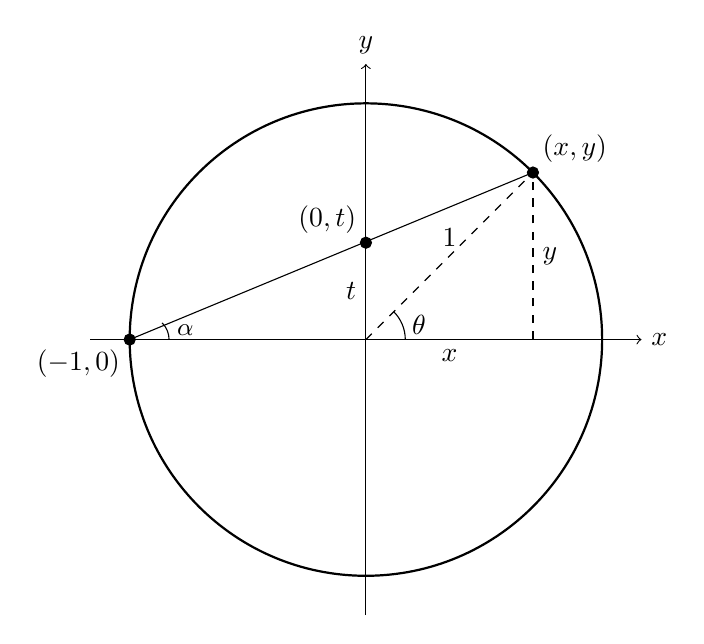
\begin{tikzpicture}
    % Draw axes
    \draw[->] (-3.5, 0) -- (3.5, 0) node[right] {$x$};
    \draw[->] (0, -3.5) -- (0, 3.5) node[above] {$y$};

    % Draw a larger unit circle (radius = 3)
    \draw[thick] (0, 0) circle (3);

    % Define angle theta
    \def\delta{45} % Angle in degrees
    \def\radius{3} % Radius of the circle

    % Calculate (x, y) point on the circle
    \pgfmathsetmacro{\x}{\radius * cos(\delta)}
    \pgfmathsetmacro{\y}{\radius * sin(\delta)}

    % Draw point (x, y) and label it
    \filldraw (\x, \y) circle (2pt) node[above right] {$(x, y)$};

    % Draw line from (x, y) to (0, t)
    \def\t{0} % Define t
    \draw (\x, \y) -- (-3, \t);

    % Draw point (-1, 0)
    \filldraw (-3, 0) circle (2pt) node[below left] {$(-1, 0)$};
    \filldraw (0, 1.23) circle (2pt) node[above left]{$(0, t)$};
    \draw (0, 0) -- (0, 1.23) node[midway, left]{$t$};
    \draw[dashed] (0, 0) -- ({3 * cos(\delta)}, {3 * sin(\delta)}) node[midway, above]{$1$};
    \draw[dashed] ({3 * cos(\delta)}, 0) -- ({3 * cos(\delta)}, {3 * sin(\delta)}) node[midway, right] {$y$};
    \draw[dashed] (0, 0) -- ({3 * cos(\delta)}, 0) node[midway, below] {$x$};
    \draw (0.5, 0) arc (0:45:0.5) node[midway, right] {$\theta$};
    \draw (-2.5, 0) arc (0:45:0.3) node[midway, right] {\small $\alpha$};
\end{tikzpicture}
\end{center}

\begin{itemize}
    \item[\quad \textbf{a.}] Express $\alpha$ in terms of $\theta$. What geometric property justifies this relationship?
    \item[\quad \textbf{b.}] What is the slope of the line $(-1, 0)$ to $(x, y)$ in terms of $t$? And in terms of $x, y$?
    \item[\quad \textbf{c.}] Express $\sin (\theta)$, $\cos{(\theta)}$ and $\tan(\alpha)$ in terms of $t$ using $x^2+y^2=1$ and the slope of part (b).
    \item[\quad \textbf{d.}] Using implicit differentiation, find $d\theta$ in terms of $t$.
    \item[\quad \textbf{e.}] Use the results from parts (c) and (d) to solve the following integral: \[\displaystyle \int \frac{1}{\sin^2{(\theta)}+\cos{(\theta)}+2} \, d\theta\]
\end{itemize}

\vspace{5mm}


\subsubsection*{IV. Extra Problems II}

\begin{itemize}
    \item[\quad \textbf{a.}] Let $P(x)$ be polynomial with real coefficients. Prove that
    \[\int_{0}^{\infty} e^{-x}P(x) \, dx=P(0)+P'(0)+P''(0)+\cdots \]
    \item[\quad \textbf{b.}] Compute the integral
    \[
   \int_{0}^{\frac{\pi}{4}} \tan^{2n}x \, dx, \quad n\ge1
    \]
\end{itemize}

\vspace{5mm}

% --------------------------------------------------------------
%     You don't have to mess with anything below this line.
% --------------------------------------------------------------

\end{document}
